\chapter{Experiments}

\section{Experimental Setup}

Three test cases are conducted to evaluate the performance of the NILM method proposed in Algorithm \ref{algorithm2}. In addition, the proposed method is compared with CO implemented in Algorithm \ref{algorithm1} and Hart's pattern recognition method. The pattern recognition method is obtained from the open-source NILM Toolkit (NILMTK) \cite{batra2014} implemented in Python. The simulation environment for the two first algorithms was the AMPL modeling language \cite{ampl} and the commercial solver CPLEX \cite{cplex}. The PC configuration was: Intel Xeon 2.4 GHz and 32 GB of memory. The only difference between the two first cases is that the reactive power is included in the second one. The third case considers a setting with a longer period and more appliances. The Almanac of Minutely Power dataset (AMPds) \cite{ampds} is chosen for evaluation. AMPds contains electricity measurements at one minute intervals. The next two subsections describe the test case's input data in depth. Furthermore, the subsection IV.C shows the two adopted metrics.

\begin{table}[tb]
\centering
\caption{Input Data for the Experimental Setup in Tests Case A and B}
\label{statesS2}
\begin{tabular}{ccccccc}
\hline
\textbf{appl} & \textbf{i} & \textbf{$D_i$} & \textbf{$\text{prev}_i$} & \textbf{$P_i$} (W) & \textbf{$Q_i$ (VAr)} & \textbf{$MD_i$} \\
\hline
    CDE            &    1              & 1            & 0            & 4606    & 413      & 20               \\
    CDE            &    2              & 1            & 1            & 252     & 413      & 5                \\
    DWE            &    3              & 2            & 0            & 751     & 34       & 5                \\
    DWE            &    4              & 2            & 0            & 478     & 0        & 15               \\
    DWE            &    5              & 2            & 0            & 136     & 34       & 15               \\
    FGE            &    6              & 3            & 0            & 129     & 6        &  7               \\
    HPE            &    7              & 4            & 0            & 37      & 17       & 30               \\
    HPE            &    8              & 4            & 0            & 1807    & 324      & 10               \\
    HPE            &    9              & 4            & 7            & 2435    & 429      & 30               \\
    WOE            &	10		 	   & 5			  & 0			 & 3442	   & 141      &  5               \\
    WOE            &	11		 	   & 5			  & 0		 	 & 3305	   & 133      &  5               \\
    WOE            &	12		 	   & 5    		  & 0		     & 2796	   & 130      &  1				 \\
    TV             &    13             & 6            & 0            & 38      & 13       & 30               \\
    TV             &    14             & 6            & 0           & 239     & 31       & 30              \\
\hline
\end{tabular}
\end{table}

\subsection{Input Data for the Test Case A and B}

The input data for the two first test cases was created with the power measurements of six appliances. These appliances are: Dryer (CDE); Dishwasher (DWE); Fridge (FGE); Heat Pump (HPE); Wall Oven (WOE); and Television/Entertainment (TVE). The full time range has 24 hours, with 1440 measurements. All the appliances are represented by 14 power states, as shown in the Table~\ref{statesS2}. Moreover, Table~\ref{statesS2} contains two columns with the previous states ($\text{prev}_i$) and the minimum number of periods ($MD_i$). Each appliance index $D_i$ and abbreviation are also informed in Table~\ref{statesS2}. These parameters in Table~\ref{statesS2} can be acquired either by: using an unsupervised approach with data from domain knowledge, laboratory tests or data aggregated measurements; or using a supervised approach with data from measurements of each appliance alone, if available. $\text{prev}_4 = 3$ which means that the state $i=4$ is allowed to be ON only after $i=3$. The window's length was chosen in order to minimize the running time. For the first two test cases, a window's length of 60 measurements was used. 

\begin{table}[t]
\centering
\caption{Input Data for the Experimental Setup in Test Case C}
\label{statesCB}
\begin{tabular}{ccccccc}
\hline
\textbf{appl} & \textbf{i} & \textbf{$D_i$} & \textbf{$\text{prev}_i$} & \textbf{$P_i$} (W) & \textbf{$Q_i$ (VAr)} & \textbf{$MD_i$} \\
\hline    
    BME      &  1          &  1      &  0         &  333           &  26        &  15            \\
    BME      &  2          &  1      &  0         &  407           &  26        &  5             \\
    CDE      &  3          &  2      &  0         &  4569 	       &  412       &  25            \\
	CDE	     &  4		   &  2	     &  3		  &  247	       &  407       &  5             \\
    DWE      &  5          &  3      &  0         &  751 	       &  34        &  3             \\
    FGE      &  6          &  4      &  0         &  129 	       &  8         &  7             \\
	FRE      &  7          &  5      &  0         &  105		   &  26	    &  20            \\
	HPE      &  8 	       &  6	     &  0		  &  37	           &  17        &  30            \\
	HPE      &  9 	       &  6	     &  0		  &  1800	       &  326       &  10            \\
	HPE      &  10		   &  6      &  0         &  2435	       &  429       &  20            \\
	TVE      &  11		   &  7	     &  0		  &  38	           &  13        &  30            \\
	TVE      &  12		   &  7	     &  0		  &  239	       &  31        &  30	         \\
\hline
\end{tabular}
\end{table}

\subsection{Input Data for the Test Case C}
The third test case considers a longer period of one week rather than one day. Hence, the total number of measurements now is 10080 measurements (one per minute). In addition, the test case C considers seven appliances: Basement Plugs and Lights (BME); Dryer (CDE); Dishwasher (DWE); Fridge (FGE); Forced Air Furnace (FRE); Heat Pump (HPE); and Television/Entertainment (TVE). All the appliances are represented by 12 power states. Table~\ref{statesCB} shows the data used as input for the model. For this test scenario, both the active and reactive power are considered. The window's length has 40 measurements.

\begin{figure*}[tb]
    \centering
    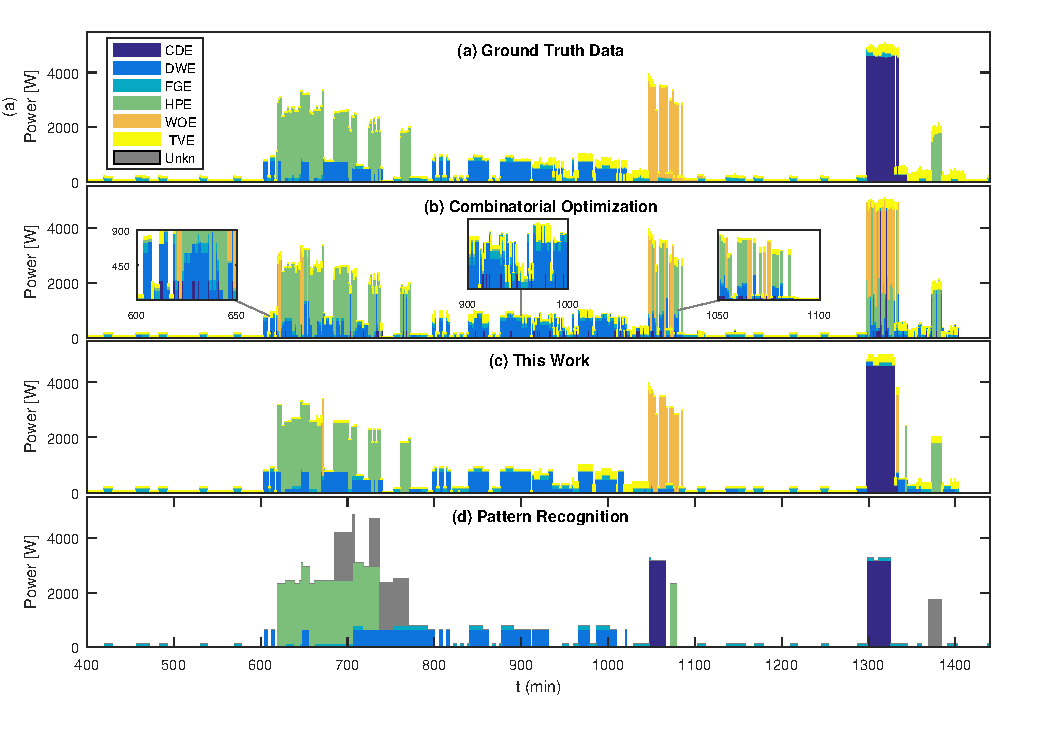
\includegraphics[width=\textwidth ]{img_test_P_2.eps}%system2.eps}
    \caption{Comparison of the real measurements (ground truth) with the proposed model and two other methods}
    \label{system2}
\end{figure*}

\subsection{Metrics}
Two metrics adapted from \cite{batra2014} are used to evaluate the accuracy of the proposed methodology. The first one will be referred as Error in Total Energy (ETE) shown in equation \eqref{metrica1}. ETE measures how well the energy consumed by each appliance was predicted. The second metric is known as Error in Assigned Power (EAP), shown in the equation \eqref{metrica2}. EAP measures how well each appliance was correctly assigned at each time slice $t$. Both metrics are normalized by the appliance's total energy consumption $y_j(t)$. The second metric provides more insight since it evaluates the correctness of the identification for each time. In other words, unlike the first metric, it does not counterbalance appliances identified at different time periods. 

\begin{equation}\label{metrica1}
   ETE_j = \dfrac{|\sum_{t}{y_j(t)} - \sum_{t}{\hat{y}_j(t)}|}{\sum_{t} { y_j(t)}}
\end{equation}

\begin{equation}\label{metrica2}
   EAP_j = \dfrac{\sum_{t} { |y_j(t) - \hat{y}_j(t)|}}{\sum_{t} { y_j(t)}}
\end{equation}


For a given appliance $j$, $y_j(t)$ is its true power measurement and $\hat{y}_j(t)$ is the predicted power at each time instant $t$. Ideally, both errors should be zero. However, it is worth mentioning that a value of zero is never achieved due to the approximation of the load signature. Hence, even in cases where the NILM algorithm detects the correct load, an error would exist. It is also worth mentioning that both metrics can achieve error rates higher than 100\%. For example, a predicted power $\hat{y}_j(t)$ higher than twice the ground truth power $y_j(t)$ can lead to such behaviour.  

\section{Tests and Results}

This section shows the results from the test cases introduced in the previous section. The MS problem is verified in CO. Also, the test case is going to be compared with Hart's pattern recognition method \cite{hart}.

\subsection{Test Case A (Active Power only)}

Results considering only the active power described in the Test Case A are discussed here. Fig.~\ref{system2} shows graphical results and compares with the two other algorithms. Table~\ref{results} shows the numerical results. The next three subtopics will discuss the behavior of each algorithm in more detail.

\subsubsection{CO Method and Verification of the MS Problem}

Fig.~\ref{system2}.b shows the disaggregation results applying only the classic CO from Algorithm \ref{algorithm1}. The highlighted zooms show a series of unrealistic activations of different loads, which is an example of the MS problem discussed in the introduction section. The first column in Table~\ref{results} shows the numerical results using the proposed metrics.  The average EAP error of the CO method is about $90\%$. 


\subsubsection{Proposed Model}
Fig.~\ref{system2}.c shows the disaggregation results using the full proposed model in the Algorithm~\ref{algorithm2}. 


%As shown in Fig. \ref{system2}.c, the multiple switching problem has been avoided by the proposed NILM method. 
The minimum time constraints \eqref{md1}-\eqref{md3} help the model to avoid multiple load switching. The second column of Table~\ref{results} shows the disaggregation results. In comparison with CO, the proposed model has a lower EAP for all loads.
%This is one of the limitations of the proposed work, since it approximates a load that is continuously switching to a continuous load.
Regarding the computational time, the usage of windows reduced the simulation time from several hours (more than 10 hours) to only a few minutes (about 3 minutes in average). FGE was the most problematic load.

\begin{table}[tb]
\centering
\caption{Error for the Case A with the Active Power Only}
\label{results}
\begin{tabular}{lcccccc}
\hline
    & \multicolumn{2}{c}{CO (\%)}                            & \multicolumn{2}{c}{This Work (\%)}                    & \multicolumn{2}{c}{Patt. Rec. (\%)}                     \\
    & \multicolumn{1}{l}{ETE} & \multicolumn{1}{l}{EAP} & \multicolumn{1}{l}{ETE} & \multicolumn{1}{l}{EAP} & \multicolumn{1}{l}{ETE} & \multicolumn{1}{l}{EAP} \\ \hline
CDE & 50.8                    & 98.2                   & 7                       & 7.3                     & 8.7                     & 84.1                    \\
DWE & 39.1                    & 89                    & 16.8                    & 29                    & 5.6                     & 74.1                    \\
FGE & 7.1                     & 70.7                    & 3.6                    & 43.9                    & 3.6                     & 53.3                    \\
HPE & 6.2                     & 57                    & 1.1                    & 5.2                    & 0.1                     & 65.9                    \\
WOE & 17.7                    & 160.1                   & 5.5                     & 15.4                    & -                       & -                       \\
TVE & 12.9                    & 55.5                    & 17.7                    & 20.7                    & -                       & -                       \\ \hline
\textbf{Average} & 22.3      & 88.41                    & 8.62                   & 20.25                   & 4.5                     & 69.35                   \\ \hline
\end{tabular}
\end{table}

\subsubsection{Comparison with Pattern Recognition}
Fig.~\ref{system2}.d shows the disaggregation results for this method. Four out of the six appliances were identified. One unknown load was also identified, which seems to be associated to the heat pump (HPE). As an example of edge dependency, the turn off event of the HPE was not detected at $t = 672$. Hence, when the load was turned on again at $t = 684$, the pattern recognition algorithm assigned the event to a different (unknown) load. The same problem also happens in the next few events and are assigned to the unknown load. The third column of the Table~\ref{results} shows the numerical results. All EAP values are over 50\%. The ETE error is lower than the other two methods; however, the ETE metric considers the energy consumption of the overall time period.

%\begin{figure}[tb]
%    \vspace{-5pt}
%    \centering
%    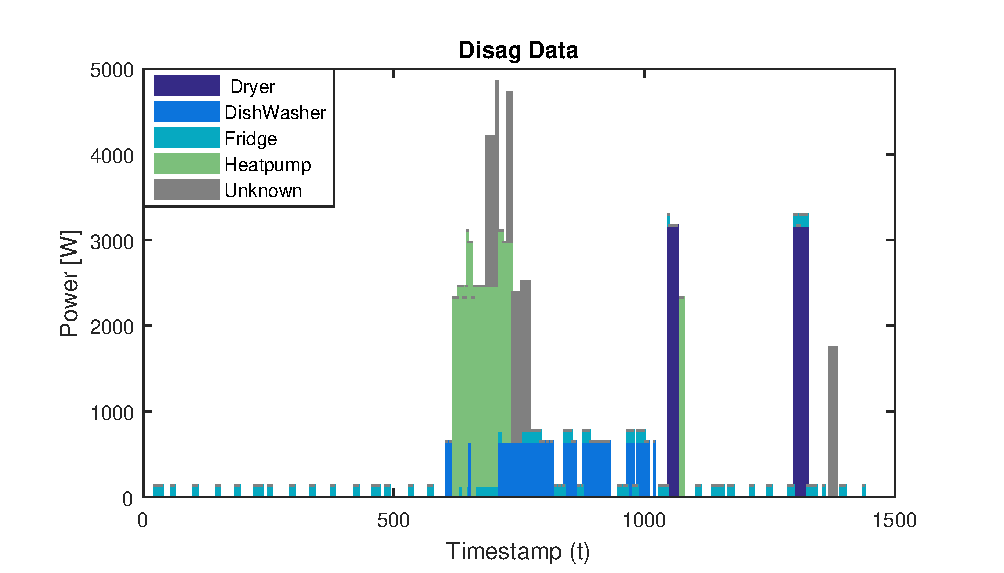
\includegraphics[width=1\columnwidth ]{results_pattern_with_unk_solo.eps}
%    \vspace{-5pt}
%    \caption{Disaggregation results applying Hart's pattern recognition algorithm.}
%    \label{hartmethod}
%\end{figure}

\subsection{Test Case B (with Reactive Power)}
The Table~\ref{results_Q} shows the numerical results when including the reactive power measurements. All the values in EAP were improved in the proposed model when comparing with the previous test case in Table~\ref{results}. Thus, the addition of new features, when available, helps on improving the method's accuracy. The average of ETE for the proposed model decreased from 8.62\% to 7\%. In addition, the average of EAP for the proposed model decreased from 20.25\% to 15.5\%. The results for CO have also highly improved from 26.65\% to 6.05\% (ETE), and from 89.7\% to 21.05\% (EAP), respectively. For pattern recognition, the same results are presented since the original method requires only reactive power.

\begin{table}[tb]
\centering
\caption{Error for the Case B Including the Reactive Power}
\label{results_Q}
\begin{tabular}{lcccccc}
\hline
    & \multicolumn{2}{c}{CO (\%)}                            & \multicolumn{2}{c}{This Work (\%)}                    & \multicolumn{2}{c}{Patt. Rec. (\%)}                     \\
    & \multicolumn{1}{l}{ETE} & \multicolumn{1}{l}{EAP} & \multicolumn{1}{l}{ETE} & \multicolumn{1}{l}{EAP} & \multicolumn{1}{l}{ETE} & \multicolumn{1}{l}{EAP} \\ \hline
CDE & 0.2                     & 0.5                     & 5.7                     & 6.1                     & 8.7                     & 84.1                    \\
DWE & 11.5                     & 28.1                    & 14                    & 23.2                    & 5.6                     & 74.1                    \\
FGE & 3.9                     & 43.5                    & 0.3                    & 28                    & 3.6                     & 53.3                    \\
HPE & 1.3                    & 5.6                    & 0.7                     & 4                     & 0.1                     & 65.9                    \\
WOE & 6.7                     & 9.5                     & 2.2                     & 12.2                    & -                       & -                       \\
TVE  & 16.1                   & 34.5                      & 19.3                    & 19.7                    & -                       & -                       \\ \hline
\textbf{Average} & 6.61       & 20.28                   & 7                     & 15.5                      & 4.5                     & 69.35                   \\ \hline
\end{tabular}
\end{table}

\subsection{Test Case C}
Table~\ref{results2} shows the numerical results for the test case C. The dataset in this case considers one more appliance than the former and a longer period of measurements. Results in Table~\ref{results2} show an EAP of 24.97\% which is almost half of the error from the other compared methods. The pattern recognition strategy identified three of the seven appliances. The most problematic appliances were DWE and FGE, with EAP of 54.7\% and 39.9\% respectively. However, error is still lower than for the other two compared methods. 

\begin{table}[tb]
\centering
\caption{Error for the Case C for a Longer Period}
\label{results2}
\begin{tabular}{lcccccc}
\hline
    & \multicolumn{2}{c}{CO (\%)}                            & \multicolumn{2}{c}{This Work (\%)}                    & \multicolumn{2}{c}{Patt. Rec. (\%)}                     \\
    & \multicolumn{1}{l}{ETE} & \multicolumn{1}{l}{EAP} & \multicolumn{1}{l}{ETE} & \multicolumn{1}{l}{EAP} & \multicolumn{1}{l}{ETE} & \multicolumn{1}{l}{EAP} \\ \hline
BME & 0.4                   & 36.8                  & 5.9                   & 22.2                  & -                    & -                    \\
CDE & 0.2                   & 2.8                   & 4.7                   & 12.2                  & 42.8                 & 52.2                   \\
DWE & 32.2                  & 109.3                   & 14.8                  & 54.7                  & -                    & -                    \\
FGE & 43.6                  & 83.2                  & 9.4                   & 39.9                  & 15.4                 & 64.1                   \\
FRE & 27                    & 27.3                  & 11.8                  & 12.2                  & -                    & -                       \\
HPE & 2.8                   & 6                   & 2.7                   & 4                   & 3.6                  & 16.1                   \\ 
TVE & 51.2                  & 94.2                  & 10                    & 29.6                  & -                    & -                    \\ \hline
\textbf{Average} & 22.48     & 51.37                  & 8.47                   & 24.97                  & 20.6                 & 44.1                 \\ \hline
\end{tabular}
\end{table}

\section{Unsupervised Tests}

\section{Analysis of Results}
This chapter presented the experiments for both the supervised and unsupervised setting. A public dataset was considered for the supervised setting while a local private dataset for the unsupervised one. As discussed in \cite{zeifman_analysis}, a good NILM algorithm should address the following six requirements: use typical meter features, minimal accuracy, no training, real-time capability, scalability, and flexibility.

The presented NILM algorithm accomplishes with most of the former requirements, since: uses only low frequency features; accomplishes the minimum 80\% requirement (considering the complement of ETE's average); the parameters in the input table make it suitable for a no training (unsupervised) setting; the results could be shown in real-time to the user at every $m$ measurements; scalability will depend on the way in which the input table is constructed and how it is updated; finally multiple appliances types are handled (multi-state, ON/OFF, constant) thanks to the parameters $MD_i$ and $prev_i$. 
